% !TeX program = pdflatex
% !BIB program = bibtex
% Template LaTeX file for DAFx-19 papers

%------------------------------------------------------------------------------------------
%  !  !  !  !  !  !  !  !  !  !  !  ! user defined variables  !  !  !  !  !  !  !  !  !  !  !  !  !  !
% Please use these commands to define title and author(s) of the paper:
\def\papertitle{Water bottle Synthesis with Modal Signal Processing}
\def\paperauthorA{Jatin Chowdhury}
\def\paperauthorB{Elliot K. Canfield-Dafilou}
\def\paperauthorC{Mark Rau}

% Authors' affiliations have to be set below

%------------------------------------------------------------------------------------------
\documentclass[twoside,a4paper]{article}
\usepackage{etoolbox}
\usepackage{dafx_20}
\usepackage{amsmath,amssymb,amsfonts,amsthm}
\usepackage{euscript}
\usepackage[latin1]{inputenc}
\usepackage[T1]{fontenc}
\usepackage{ifpdf}
% \usepackage{subfigure}
\usepackage{subcaption}

\usepackage[english]{babel}
\usepackage{caption}
% \usepackage{subfig} % or can use subcaption package
\usepackage{xcolor}
\usepackage{soul}
\usepackage{cite}


\input glyphtounicode
\pdfgentounicode=1

\setcounter{page}{1}
\ninept

% build the list of authors and set the flag \multipleauth to handle the et al. in the copyright note (in DAFx_20.sty)
%==============================DO NOT MODIFY =======================================
\newcounter{numauth}\setcounter{numauth}{1}
\newcounter{listcnt}\setcounter{listcnt}{1}
\newcommand\authcnt[1]{\ifdefined#1 \stepcounter{numauth} \fi}

\newcommand\addauth[1]{
\ifdefined#1 
\stepcounter{listcnt}
\ifnum \value{listcnt}<\value{numauth}
\appto\authorslist{, #1}
\else
\appto\authorslist{~and~#1}
\fi
\fi}
%======DO NOT MODIFY UNLESS YOUR PAPER HAS MORE THAN 10 AUTHORS========================
%==we count the authors defined at the beginning of the file (paperauthorA is mandatory and already accounted for)
\authcnt{\paperauthorB}
\authcnt{\paperauthorC}
\authcnt{\paperauthorD}
\authcnt{\paperauthorE}
\authcnt{\paperauthorF}
\authcnt{\paperauthorG}
\authcnt{\paperauthorH}
\authcnt{\paperauthorI}
\authcnt{\paperauthorJ}
%==we create a list of authors for pdf tagging, for example: paperauthorA, paperauthorB, ... and paperauthorF (last author)
\def\authorslist{\paperauthorA}
\addauth{\paperauthorB}
\addauth{\paperauthorC}
\addauth{\paperauthorD}
\addauth{\paperauthorE}
\addauth{\paperauthorF}
\addauth{\paperauthorG}
\addauth{\paperauthorH}
\addauth{\paperauthorI}
\addauth{\paperauthorJ}
%====================================================================================

\usepackage{times}
% Saves a lot of ouptut space in PDF... after conversion with the distiller
% Delete if you cannot get PS fonts working on your system.

% pdf-tex settings: detect automatically if run by latex or pdflatex
\newif\ifpdf
\ifx\pdfoutput\relax
\else
   \ifcase\pdfoutput
      \pdffalse
   \else
      \pdftrue
\fi

\ifpdf % compiling with pdflatex
  \usepackage[pdftex,
    pdftitle={\papertitle},
    pdfauthor={\paperauthorA},
    colorlinks=false, % links are activated as colror boxes instead of color text
    bookmarksnumbered, % use section numbers with bookmarks
    pdfstartview=XYZ % start with zoom=100% instead of full screen; especially useful if working with a big screen :-)
  ]{hyperref}
  \pdfcompresslevel=9
  \usepackage[pdftex]{graphicx}
%   \usepackage[figure,table]{hypcap}
\else % compiling with latex
  \usepackage[dvips]{epsfig,graphicx}
  \usepackage[dvips,
    colorlinks=false, % no color links
    bookmarksnumbered, % use section numbers with bookmarks
    pdfstartview=XYZ % start with zoom=100% instead of full screen
  ]{hyperref}
  % hyperrefs are active in the pdf file after conversion
  % \usepackage[figure,table]{hypcap}
\fi
\usepackage[hypcap=true]{caption}

% My packages
\usepackage{tikz}
\usepackage{tkz-euclide}
\usetkzobj{all}
\usepackage{cleveref}

\usepackage{listings}
\definecolor{codegreen}{rgb}{0,0.6,0}
\definecolor{codegray}{rgb}{0.5,0.5,0.5}
\definecolor{codepurple}{rgb}{0.58,0,0.82}
\definecolor{backcolour}{rgb}{0.95,0.95,0.92}
 
\lstdefinestyle{mystyle}{
    backgroundcolor=\color{backcolour},   
    commentstyle=\color{codegreen},
    keywordstyle=\color{magenta},
    numberstyle=\tiny\color{codegray},
    stringstyle=\color{codepurple},
    basicstyle=\footnotesize,
    columns=flexible,
    breakatwhitespace=false,         
    breaklines=true,                 
    captionpos=b,                    
    keepspaces=true,                               
    showspaces=false,                
    showstringspaces=false,
    showtabs=false,                  
    tabsize=4
}
 
\lstset{style=mystyle}

\DeclareMathAlphabet{\mathpzc}{OT1}{pzc}{m}{it}
\newcommand{\z}{\mathpzc{z}}

\title{\papertitle}

\affiliation{
\paperauthorA, \paperauthorB \, and \paperauthorC \, }
{\href{http://ccrma.stanford.edu}{Center for Computer Research in Music and Acoustics} \\ Stanford University \\ Stanford, CA, USA \\ {\tt\{jatin|kermit|mrau\}@ccrma.stanford.edu}}

\begin{document}
% more pdf-tex settings:
\ifpdf % used graphic file format for pdflatex
  \DeclareGraphicsExtensions{.png,.jpg,.pdf}
\else  % used graphic file format for latex
  \DeclareGraphicsExtensions{.eps}
\fi

\maketitle
%
\begin{abstract}
We present a method for accurately synthesizing the acoustic response
of a water bottle using modal signal processing. We start with extensive measurements of two water bottles with considerations for how the level of water inside the bottles, the number and placement of stickers attached to the exterior
of the bottles, and the method of striking the bottles affect their sound. We perform modal analysis of these measurements and implement  a real-time modal water bottle synthesizer.
\end{abstract}

\section{Introduction} \label{sec:intro}
%
Previous work has examined the use of modal signal processing
for synthesizing carillon bells \cite{canfielddafilou:werner:bellEffects:2017,
rau:das:canfielddafilou:carillon:2019}, artificial reverberation 
\cite{abel2014a}, cymbal synthesis \cite{travis_cymbals}, and more 
\cite{abel_kurt_modal,rocket-bells}. This work builds on the previous
research to use modal synthesis for the accurate modelling of water bottle 
acoustics.

Although most water bottles are not designed to function primarily as musical
instruments, the authors have noticed that certain water bottles
can produce a pleasing resonant sound when struck with a knee, hand,
or other body part. The authors further noticed that water bottles can
produce a great variety of sounds, depending not only on the shape and
material of the bottle, but also on the amount of liquid contained
within the bottle, as well as the amount and placement of stickers on the
exterior of the bottle. Water bottle acoustics have not gone unnoticed
by water bottle manufacturers, as at least one prominent manufacturer claims
to be well aware of the pleasing acoustic properties of their bottles
\cite{hydroflask_email}.

There exists considerable physics literature concerning the harmonic
responses of various liquid containers and other thin-shell objects.
Previous research has often focused on the modal behaviour of wine
glasses and beer bottles, particularly with regard to the fundamental
frequency at which the container vibrates \cite{russelBEER,french1983vino,
chen2005does,rossing1990wine,jundt2006vibrational}. Others focus particularly
on the behavior of containers filled with heated beverages, such as
coffee or hot chocolate \cite{crawford1982hot,morrison2002sound,
morrison2014acoustics}.
% Not sure if we need these ones...
% \cite{thines2012wine} discusses the pitch
% and sound of a shattering wine glass, while \cite{piacsek2015glass}
% examines how mass loading affects the resonant structure of a wine glass.
\cite{courtois2008tuning} gives consideration to how liquid is distributed
within a glass, while \cite{apfel1982whispering} examines the circular
capillary waves on the surface of the liquid of a resonating wine glass.
Finally, the authors of \cite{arbel2017wine} explored the sympathetic
resonance generated in a wine glass coupled to a vibrating string.

% https://research.cs.cornell.edu/HarmonicShells/HarmonicShells09.pdf
% https://www.springer.com/gp/book/9783642164071
% we should probably cite helmholtz 
% \cite{russelBEER} modes of beer bottle
% the following two citations are nicely described here: http://www.kilty.com/coffee.htm
% \cite{french1983vino} wine glass pitch
% \cite{chen2005does} wine glass pitch
% \cite{rossing1990wine} comparison of wine glasses to bells
% \cite{bragg1921world} pitch change noticed in beer glass
% \cite{crawford1982hot} pitch change in hot chocolate
% \cite{morrison2002sound} modes of coffee cup change with bubbles in instant coffee % https://acoustics.org/pressroom/httpdocs/143rd/Rossing.html
% \cite{morrison2014acoustics} acoustic concepts demonstrated with coffee cup
% \cite{thines2012wine} pitch and sound of shattering wine glass
% \cite{piacsek2015glass} mass loading the resonant structure of a wine glass with liquid
% \cite{jundt2006vibrational} vibrational modes of wine glass with different levels of liquid
% \cite{courtois2008tuning} how the liquid is distributed in the glass matters (this is out in for the maple syrup)
% \cite{apfel1982whispering} exploration of circular capillary waves on the surface of the liquid when exciting wine glass with wet finger
% \cite{arbel2017wine} for some reason these people coupled a vibrating string to a wine glass to make it resonate sympathetically... really not sure why :D


%  hydroflask is made of high quality food grade 18/8 stainless steel, but they're vacuum insulated and with "custom powdered coat"
% some materials properties: https://www.theworldmaterial.com/what-is-18-8-stainless-steel/

We take measurements from a 32 oz. Wide Mouth
HydroFlask,\footnote{\url{https://www.hydroflask.com/32-oz-wide-mouth/}}
compared to the water bottle given to attendees of the 2019 DAFx
conference (seen in ~\Cref{fig:dafx_measure}), measured containing different amounts of water and with different placements of stickers on the exteriors of the
bottles.

The structure of the paper is as follows: in \S\ref{sec:measure} we describe
our water bottle acoustical measurement procedure. \S\ref{sec:analysis}
contains modal analysis of the water bottle measurement data.
Finally in \S\ref{sec:results} we discuss our results, and the
implementation of a full water bottle synthesizer.


\begin{figure}[!t]
    \centering
    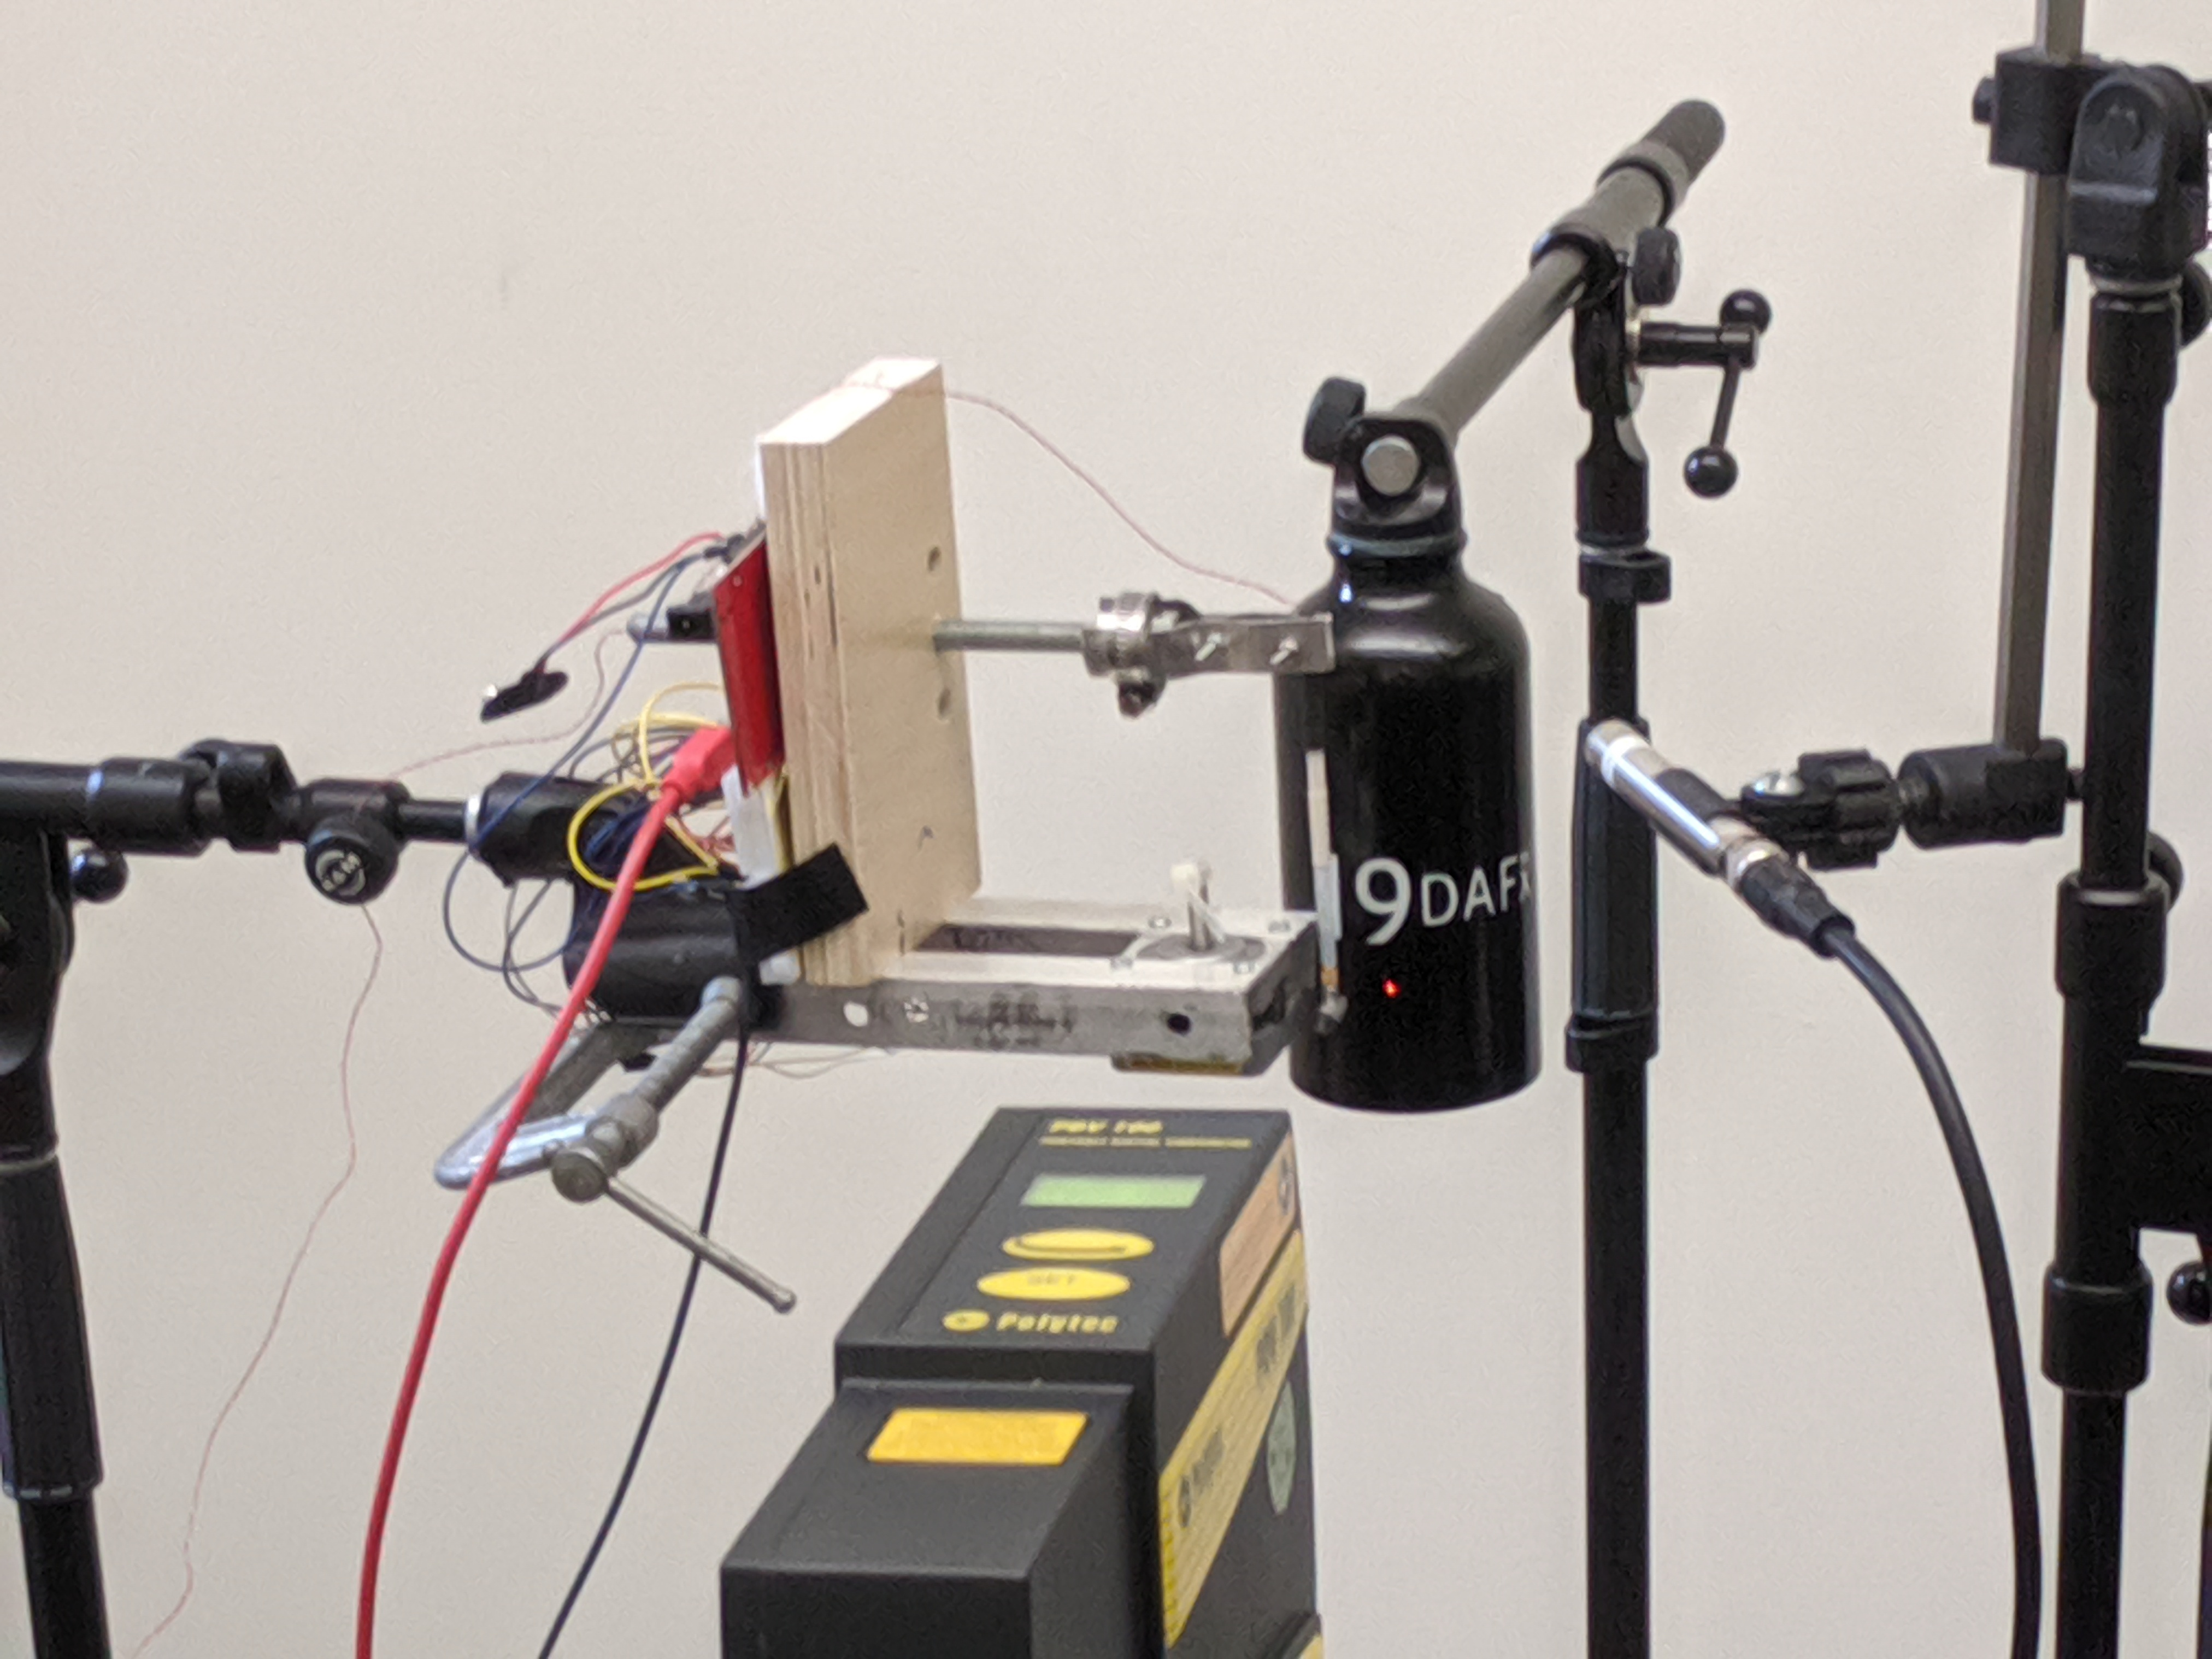
\includegraphics[width=3in]{Figures/dafx_measure}
    \caption{\it{Measurement setup for the DAFx water bottle}}
    \label{fig:dafx_measure}
\end{figure}

\section{Measurements} \label{sec:measure}
%
We wish to study the vibrational modes of the water bottle independent of the method by which it is struck. To do this, we strike the water bottle with a force sensing hammer and measure the surface velocity of the water bottle at a corresponding point using a laser Doppler vibrometer. We additionally captured the near field radiation using a pressure microphone. From both these measurements, we deconvolve out of the signal the impact of the force hammer. The full setup can be seen in \Cref{fig:dafx_measure}. We also used a scanning vibrometer to observe the mode shapes and gain further insight into the vibrational characteristics of the bottles. 

We made measurements of both a 32 oz. Wide Mouth HydroFlask and the complimentary DAFx19 water bottles with no water as well as $1/32$, $1/16$, $1/8$, $1/4$, $1/2$, and full with water. We additionally made measurements of the HydroFlask with the exterior covered in vinyl stickers as well as several intermediate and differently placed amounts of stickers. 


\begin{figure*}
    \centering
    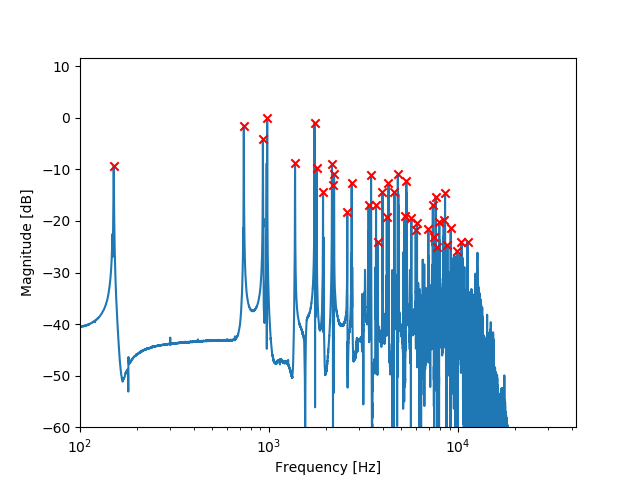
\includegraphics[width=2.25in,trim={0 0 1cm 1cm},clip]{../Figures/ModePick_ex}
    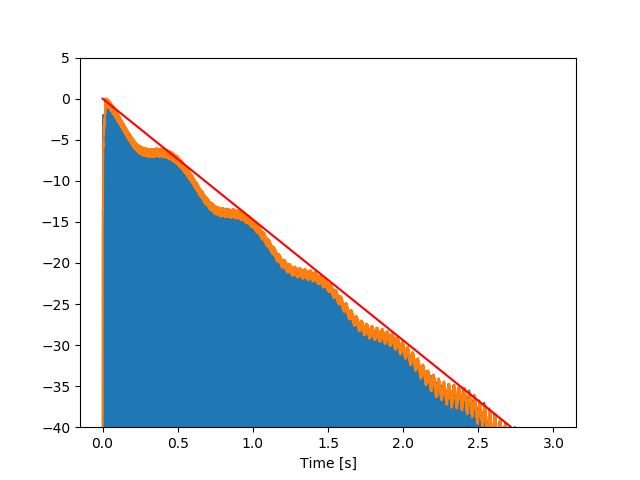
\includegraphics[width=2.25in,trim={0 0 1cm 1cm},clip]{../Figures/DecayFit_ex}
    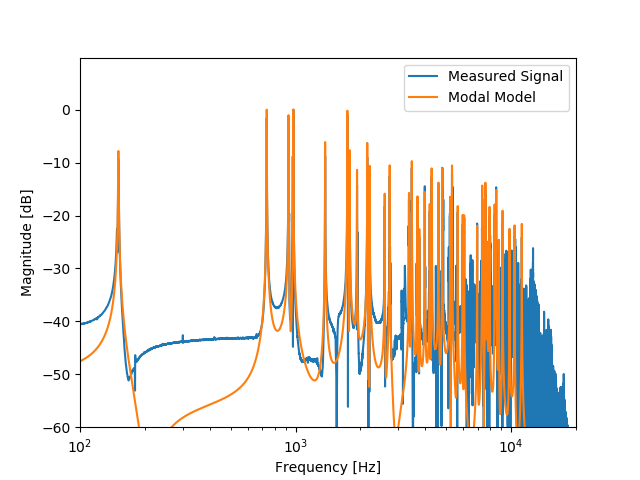
\includegraphics[width=2.25in,trim={0 0 1cm 1cm},clip]{../Figures/Model_ex}
    \caption{\it{Modal analysis pipeline: (left) picking the mode frequencies,
    (center) estimating the decay rate of a single mode,
    (right) using a least-squares fit to estimate the complex
    amplitudes of the modes that ideally resynthesize the
    original signal.}}
    \label{fig:modal_analysis}
\end{figure*}

Finally, we also wanted some understanding of different impacts on the water bottles. To make these measurements, we adhered an accelerometer to the inside of the HydroFlask and struck the outside (at the location of the accelerometer) with a variety of drum mallets and body parts.  



%
% \begin{figure}[!htb]
%     \centering
%     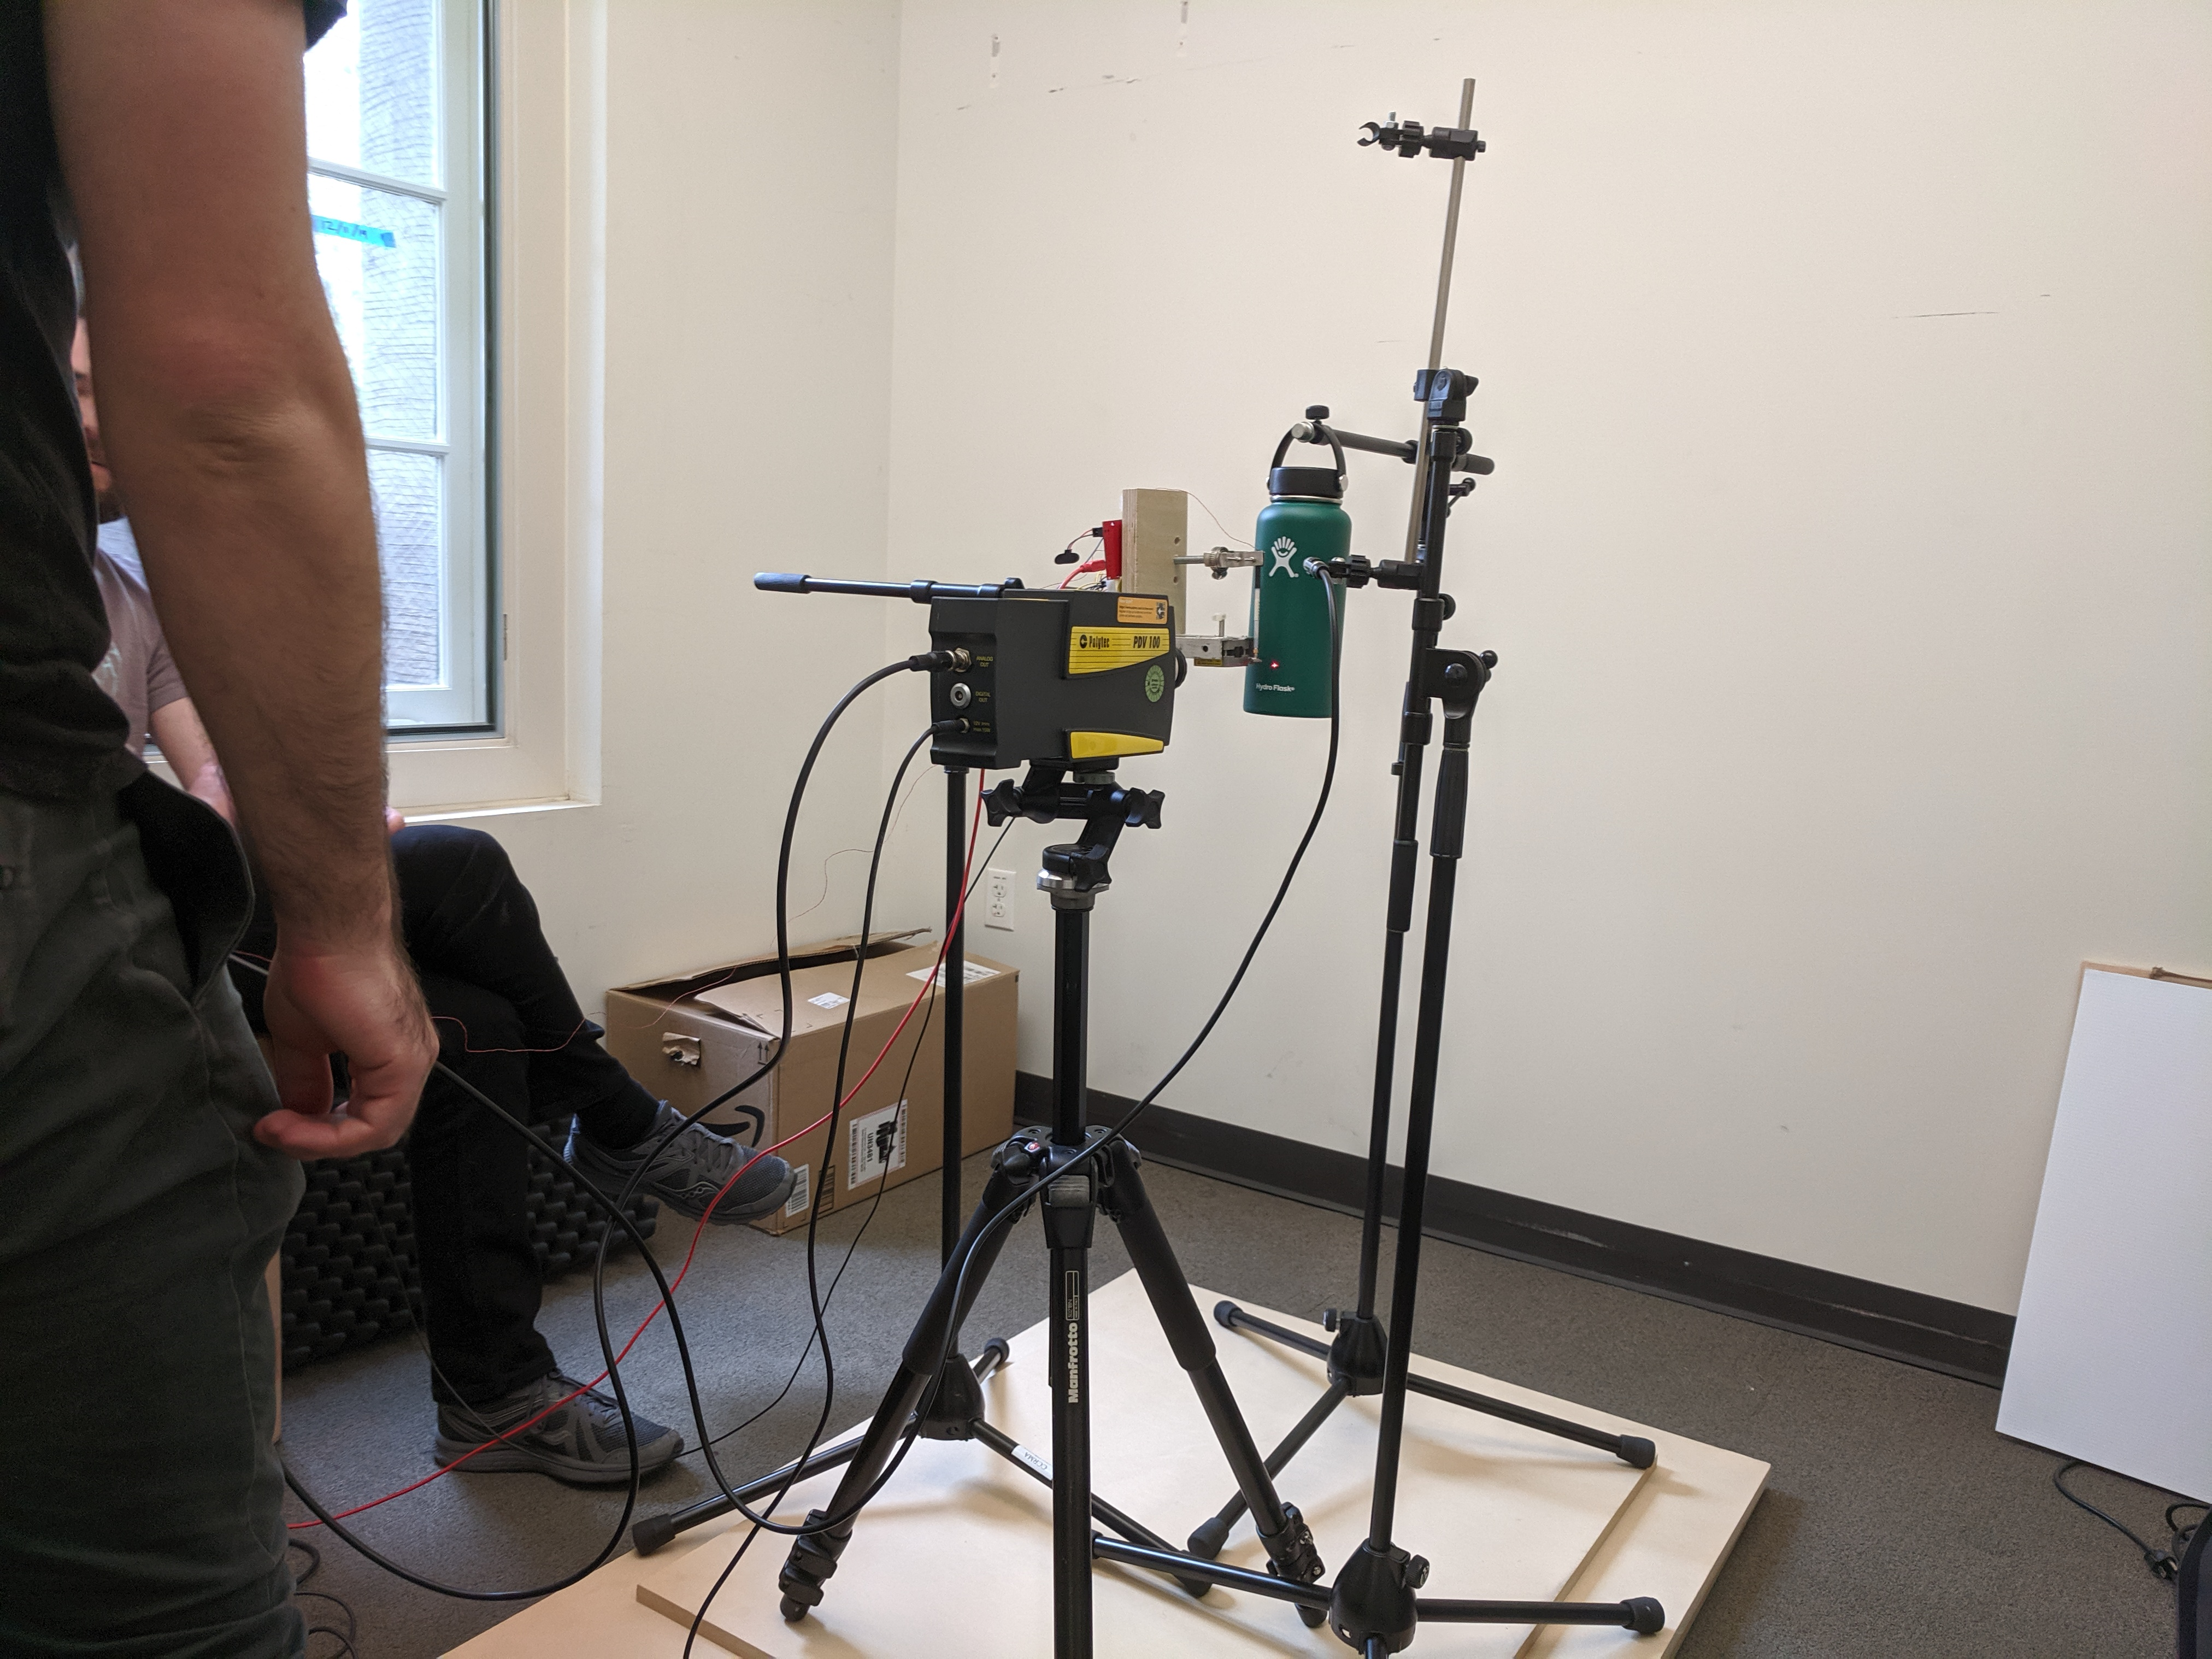
\includegraphics[width=3in]{Figures/hydroflask_measure}
%     \caption{\it{Measurement setup for the HydroFlask water bottle}}
%     \label{fig:hydro_measure}
% \end{figure}
%



\section{Analysis} \label{sec:analysis}


\subsection{Modal Analysis} \label{sec:modal-analysis}
%
Similar to the carillon bells modelled in \cite{canfielddafilou:werner:bellEffects:2017,rau:das:canfielddafilou:carillon:2019},
we can use modal analysis to model the water bottle sounds as
a sum of exponentially decaying sinusoids,
\begin{equation}
    y(t) = \sum_{m=1}^M \alpha_m e^{j\omega_m t} e^{-t/\tau_m} \,,
    \label{eq:modal-def}
\end{equation}
%
where $\alpha_m$ is the complex amplitude, $\omega_m$ is the mode
frequency, and $\tau_m$ is the decay rate for each mode $m$.

For modal analysis we use the helper functions
provided by the \texttt{Python} audio signal processing library
\texttt{audio\_dspy}.\footnote{\url{https://github.com/jatinchowdhury18/audio_dspy}}
This process involves the following steps:
\begin{enumerate}
    \item Picking the modal frequencies from the original recording.
    \item Estimate the decay rate of each mode.
    \item Estimate the complex amplitude of each mode.
\end{enumerate}
%
The steps of the process are shown in  full in \Cref{fig:modal_analysis}.

For finding the mode frequencies, we use a simple peak-picking
algorithm over the Fourier Transform of the original signal.

For estimating the mode decay rates, we begin by filtering
the signal using a 4th order Butterworth bandpass filter
centered on the mode frequency, with a bandwidth of 30 Hz.
We then apply a Root-Mean-Squared level detector as defined
in \cite{giannoulis2012compressor} to estimate the energy
envelope of the mode. Finally, we use a linear regression
to estimate the slope of the energy envelope (measured in
decibels per sample).

After computing the mode frequencies and decay
rate, we perform a simple least squares fit to
estimate the complex amplitude of each mode that
most accurately resynthesizes the original recording.

\begin{figure}[t]
\centering
    \begin{subfigure}[b]{\columnwidth}
         \centering
         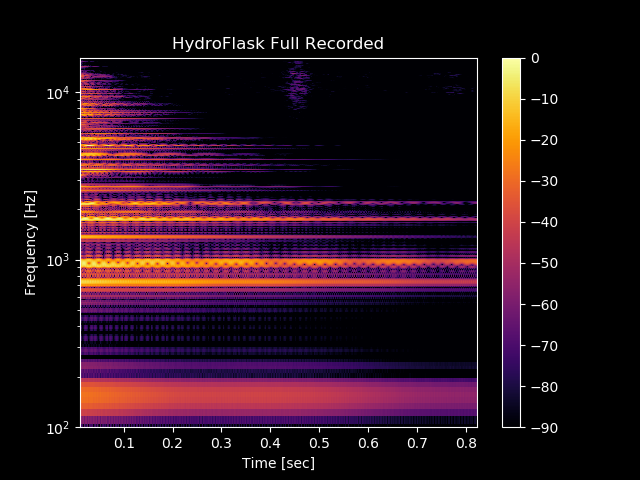
\includegraphics[width=\linewidth,trim={0 0 1.5cm 0.5cm},clip]{../Figures/Specgrams/HydroFlask Full Recorded.png}
         \caption{Recorded}
    \end{subfigure}
    \begin{subfigure}[b]{\columnwidth}
         \centering
         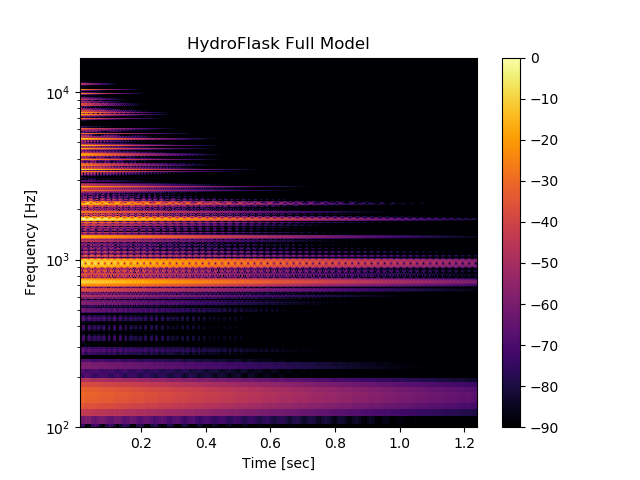
\includegraphics[width=\linewidth,trim={0 0 1.5cm 0.5cm},clip]{../Figures/Specgrams/HydroFlask Full Model.png}
         \caption{Resynthesized}
    \end{subfigure}
    \caption{\it{Spectrograms of the full HydroFlask recorded (above) and resynthesized (below).}}
    \label{fig:hydroflask-specs}
\end{figure}
%
\subsection{Modal Resynthesis} \label{sec:synthesis}
%
For synthesizing the modes we use the Max Matthews
phasor filter, as introduced in \cite{phasorfilter}.
This filter is described by the difference equation:
\begin{equation}
    y_m[n] = \alpha_m x[n] + e^{j\omega_m} e^{-1/\tau_m} y_m[n-1]
    \label{eq:phasor}
\end{equation}
%
where $\tau_m$ is the mode decay rate described above,
$\alpha_m$ is the complex amplitude of the mode, and $\omega_m$
is the mode frequency. This filter structure is known for
having favorable numerical properties, as well as for being
stable regardless of real-time parameter modulation.
While the output of the filter is complex, a real signal can
be constructed by taking either the real or imaginary part of
the output signal (the two parts will be identical aside from
a quarter-cycle phase shift). The results of the resynthesis
process can be seen in \cref{fig:hydroflask-specs}.

\subsection{Water Level Analysis} \label{sec:water}
%
Next we examine the how the modal response of the water bottle
changes as the water level in the water bottle changes. 
%
\subsubsection{Frequency Variation} \label{sec:water-freq}
%
% Measurements of the HydroFlask bottle show that as the water
% level increases, the first mode frequency increases, while the
% higher modes stay at the same frequency. \hl{This makes physical
% sense since the lowest mode frequency corresponds to the Helmholtz
% resonance of the bottle, and changing the water level
% effectively decreases the size of the air column inside the
% bottle, thereby causing the lowest mode frequency to increase
% (@TODO: ask Mark if this is correct).}

Measurements of the HydroFlask bottle show that as the water
level increases, the first mode frequency decreases, while the
higher modes stay at the same frequency. This suggests that the higher frequency modes are associated with vibration similar to that of a cylindrical shell, while the lowest frequency resonance is more similar to that of a beam clamped at one end with an additional mass at the end \cite{qatu2004vibration}. Figure~\ref{fig:scans} shows vibrometer scans of the HydroFlask filled roughly 40\% with water as well as empty for three different mode shapes. The scans support the model hypothesis as the frequency of two higher shell modes are similar, while the frequency of the lowest beam-like mode decreases in frequency with added mass. The measured frequency responses for the HydroFlask filled with different levels of water can be seen in fig.~\ref{fig:hydro-different-water-levels}.

\begin{figure}[!t]
    \centering
    \begin{subfigure}[b]{.32\columnwidth}
         \centering
         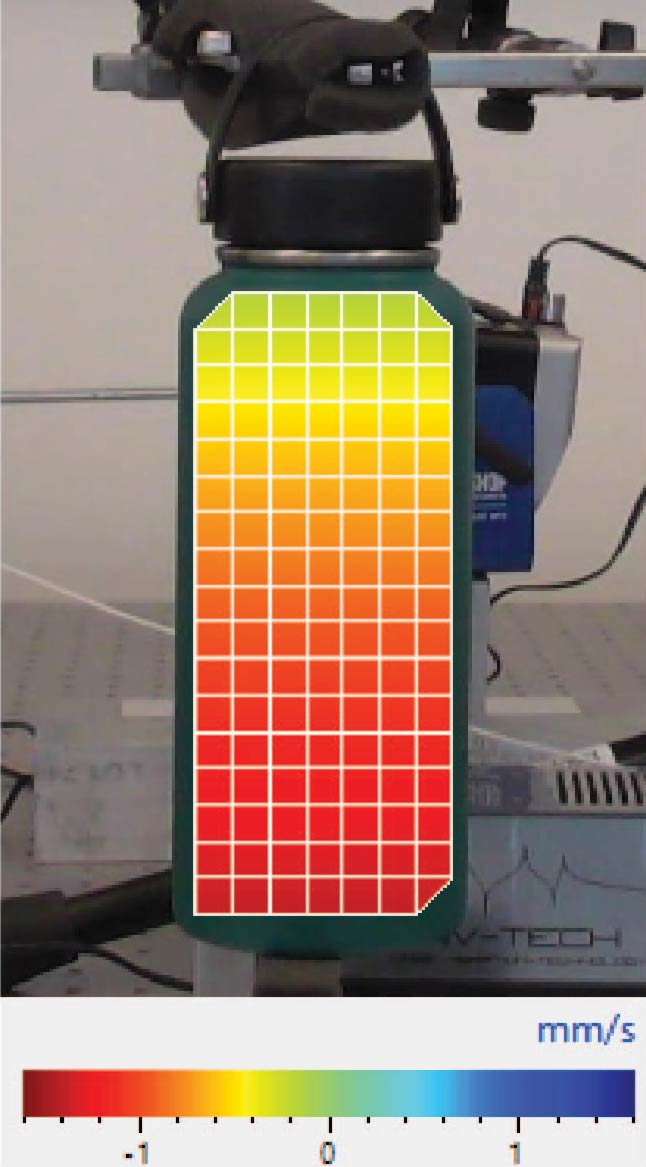
\includegraphics[width=\columnwidth]{Paper/Figures/Water_157_5.jpg}
         \caption{157.5\ Hz}
    \end{subfigure}
    \begin{subfigure}[b]{.32\columnwidth}
         \centering
         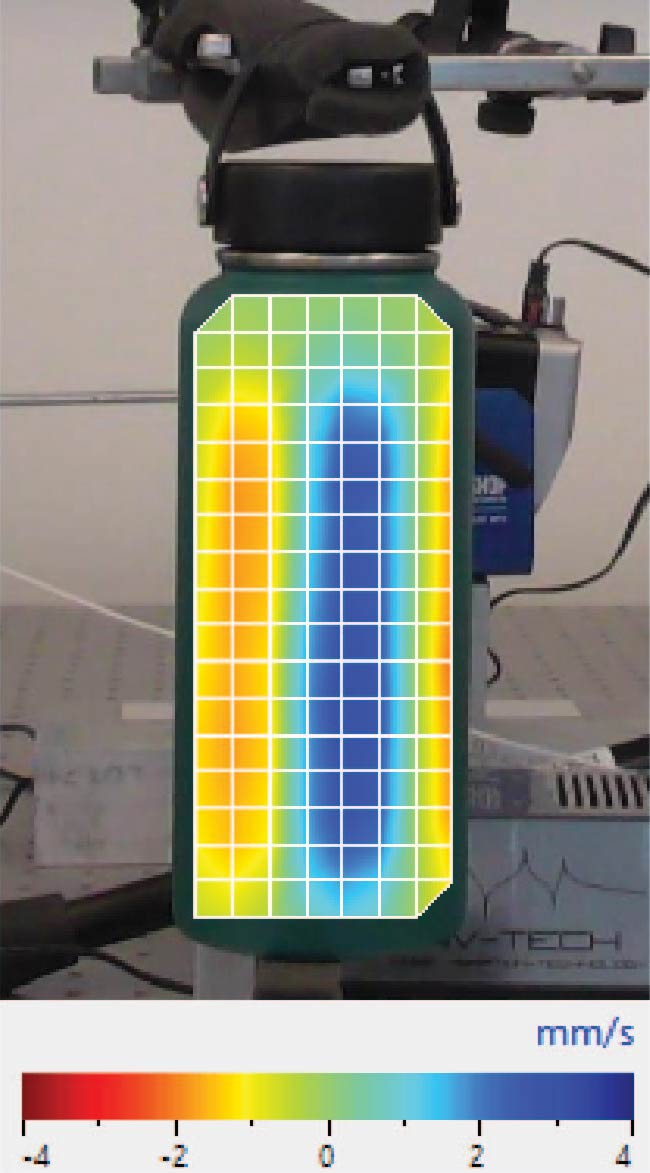
\includegraphics[width=\columnwidth]{Paper/Figures/Water_735_6.jpg}
         \caption{735.6\ Hz}
    \end{subfigure}
    \begin{subfigure}[b]{.32\columnwidth}
         \centering
         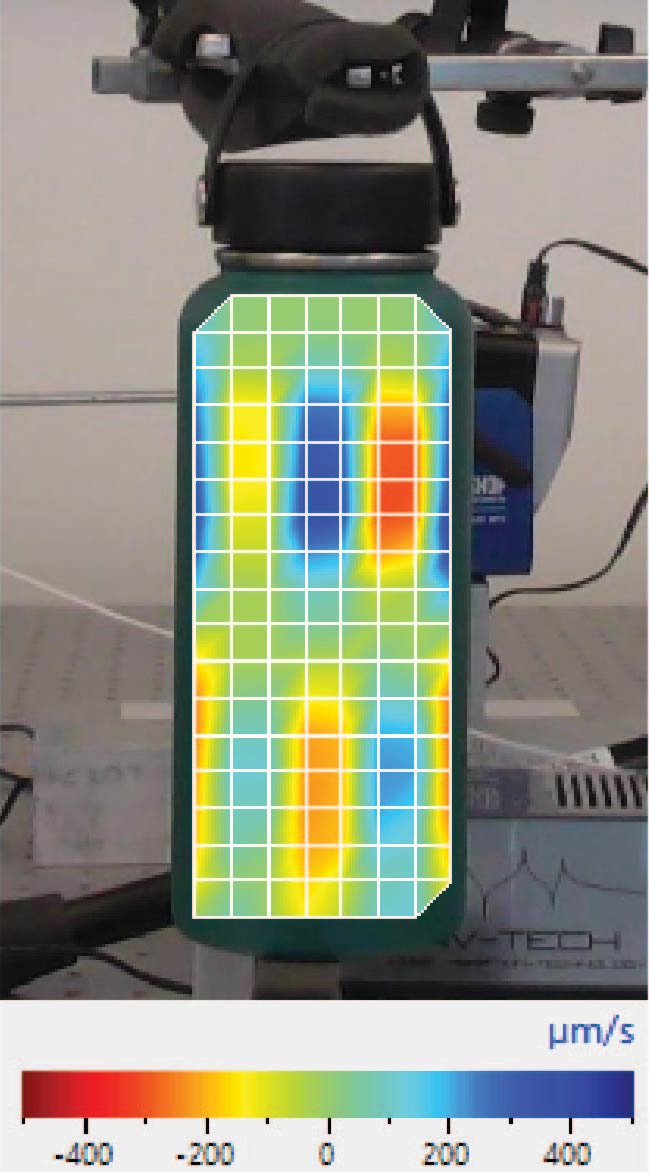
\includegraphics[width=\columnwidth]{Paper/Figures/Water_1780.jpg}
         \caption{1780\ Hz}
    \end{subfigure}
    \begin{subfigure}[b]{.32\columnwidth}
         \centering
         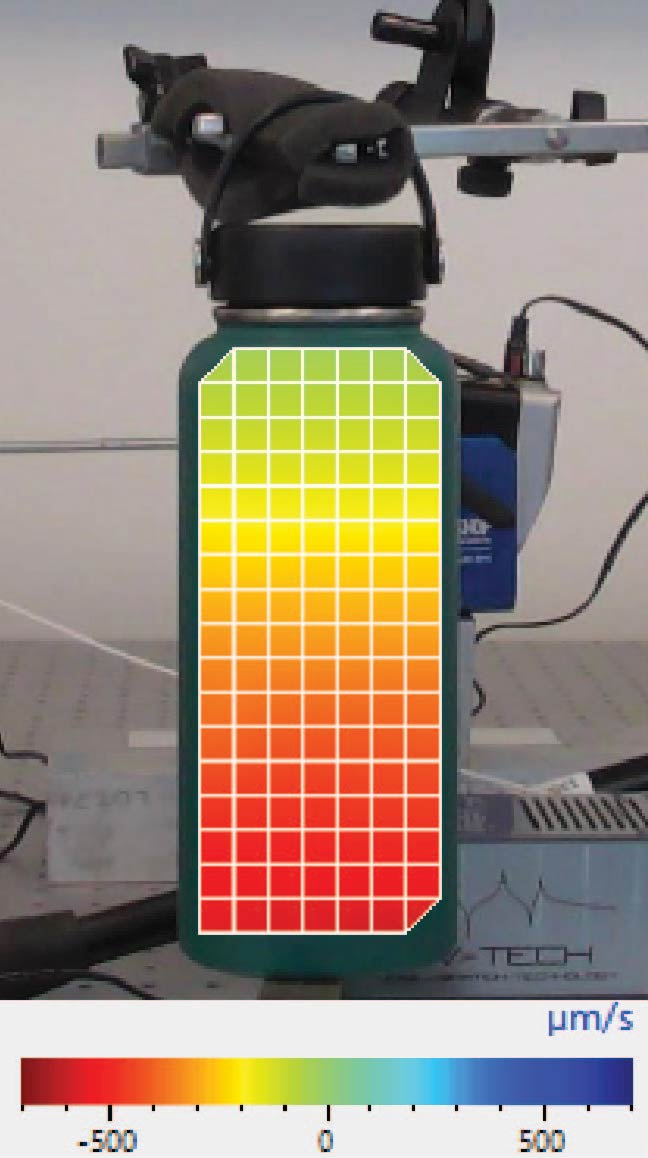
\includegraphics[width=\columnwidth]{Paper/Figures/NoWater_219_4.jpg}
         \caption{219.4\ Hz}
    \end{subfigure}
    \begin{subfigure}[b]{.317\columnwidth}
         \centering
         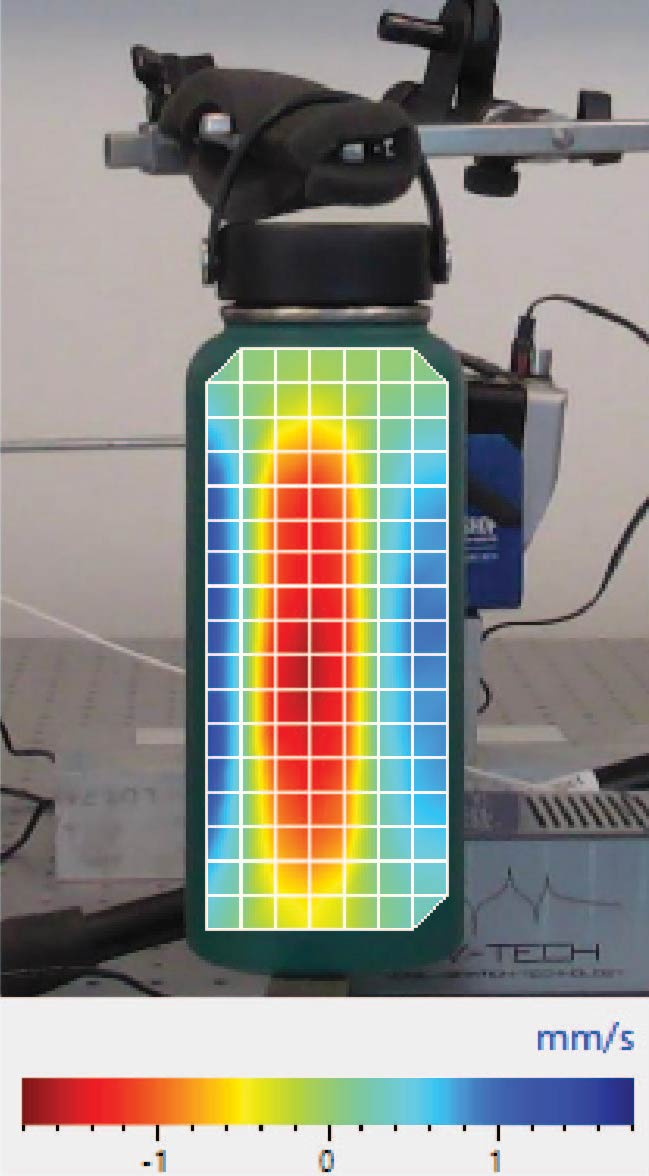
\includegraphics[width=\columnwidth]{Paper/Figures/NoWater_731_3.jpg}
         \caption{731.3\ Hz}
    \end{subfigure}
    \begin{subfigure}[b]{.32\columnwidth}
         \centering
         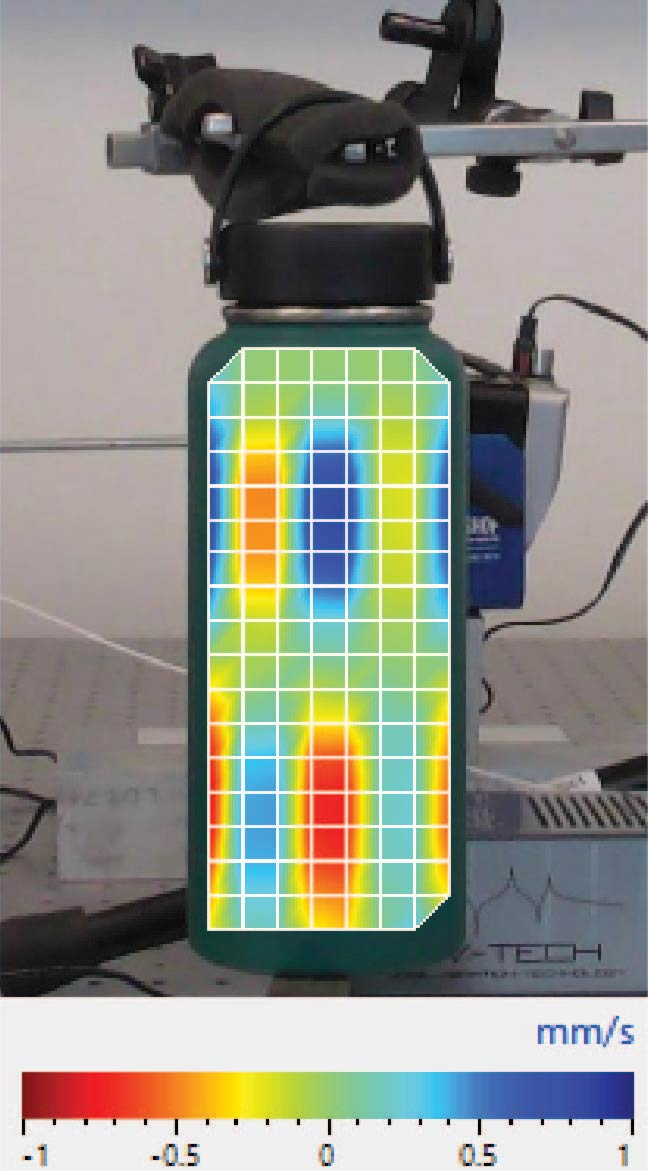
\includegraphics[width=\columnwidth]{Paper/Figures/NoWater_1780.jpg}
         \caption{1780\ Hz}
    \end{subfigure}
    
    \caption{\it{Vibrometer scans without (bottom) and with roughly 40 \% water (top).}}
        \label{fig:scans}
\end{figure}

%
\begin{figure}[!t]
    \centering
    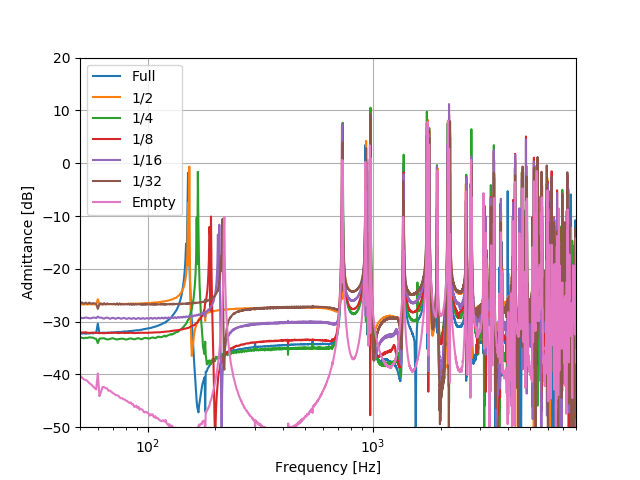
\includegraphics[width=\linewidth,trim={0 0 1cm 1cm},clip]{../Figures/DifferentLevels/HydroWaterLevelsAdmitt}
    \caption{\it{Admittance of the HydroFlask with different amounts of water.}}
    \label{fig:hydro-different-water-levels}
\end{figure}
%
We can model the dependence between the frequency of the
first mode and the water level using a modified sigmoid
function of the form:
\begin{equation}
    f(x) = C \left(1 - \frac{1}{1 + \exp(-b(x-a))} \right) + d
    \label{eq:mod_sigmoid}
\end{equation}

A comparison of the model with the measured data can be seen in \Cref{fig:water-mode-freq}.
%
\begin{figure}[!htb]
    \centering
    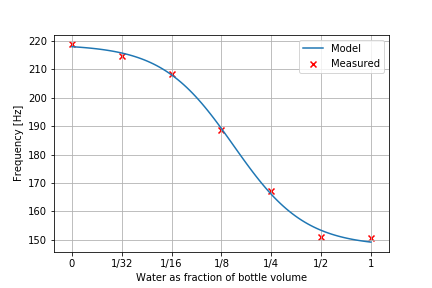
\includegraphics[width=\linewidth,trim={0 0 1cm 1cm},clip]{../Figures/Water_Freq}
    \caption{\it{Variation of the first mode frequency of the HydroFlask
                with the amount of water in the bottle}}
    \label{fig:water-mode-freq}
\end{figure}
%
\subsubsection{Damping Variation} \label{sec:water-damp}
%
Further analysis shows that the damping of the lowest two modes
varies with water level as well (see \cref{fig:hydro-different-water-levels}). We can similarly model the
variation of the mode decay rates with water level, using a
5-th order polynomial to fit the decay rates of the first
two modes (see \Cref{fig:water-mode-damp}). Note that the dampings
of the first two modes can be modelled separately, however we chose
to use a combined model due to the rough similarity between the
two separate models. The water level has very little impact on the dampings of the higher modes. This supports the hypothesis presented in \S\ref{sec:water-freq} that the lowest modes are beam-like modes while the higher modes are cylindrical shell-like modes, as the mass loading disproportionately affects the beam-like modes. 
%
\begin{figure}[!t]
    \centering
    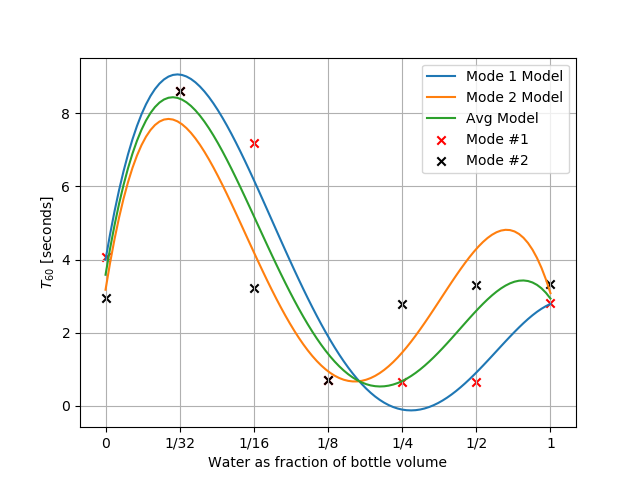
\includegraphics[width=\linewidth,trim={0 0 1cm 1cm},clip]{../Figures/Water_Damping}
    \caption{\it{Variation of the first two modes decay rates
                 with the amount of water in the HydroFlask}}
    \label{fig:water-mode-damp}
\end{figure}
%
\subsection{Sticker Analysis} \label{sec:sticker}
%
Initially, we compared two 32 oz. HydroFlask water bottles, one
with stickers, one without, and noted that they had markedly different
timbres. We then proceeded to take measurements of the
bottle covered in varying amount of (removable) vinyl stickers. We found
that the mode frequencies remained mostly unchanged with the
addition of stickers, however, the mode dampings had noticeable
variations (see \cref{fig:sticker-mode-damp}). Much like a moon gel on a drum head, a small application of stickers dramatically increases the damping. Adding a larger amount of stickers naturally increases the damping, although it has a less pronounced effect than the difference between no stickers and some stickers. 
%
\begin{figure}[!htb]
    \centering
    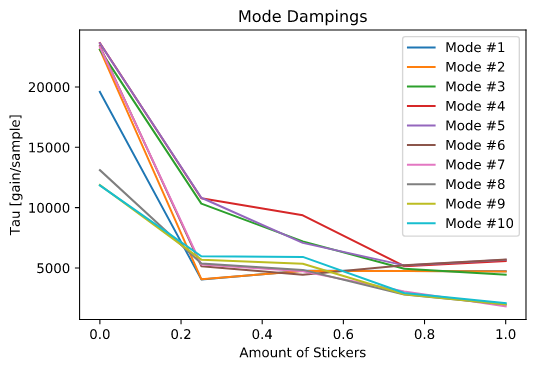
\includegraphics[width=\linewidth,trim={0 0 1cm 1cm},clip]{../Figures/StickerDamping}
    \caption{\it{Variation of the first ten modes decay rates
                 with the amount of stickers on the HydroFlask}}
    \label{fig:sticker-mode-damp}
\end{figure}
%
\subsection{Swinging Vibrato} \label{sec:swing}
%
When a water bottle is struck in such a way to produce an acoustic
response, it often swings back and forth a little bit. This swinging
causes the water within the bottle to move with the swinging, thereby
causing some of the lower mode frequencies to oscillate (see
\Cref{fig:swinging-vibrato}). This oscillation
manifests itself perceptually as a sort of vibrato effect. In
order to model this ``swinging vibrato'' we use the following
steps:
\begin{enumerate}
    \item Measure (or estimate) the height of the bottle.
    \item Calculate the swinging frequency of the bottle.
    \item Synthesize an initial amplitude and damping factor
        for the swinging oscillations.
\end{enumerate}
%
\subsubsection{Bottle Height}
%
In cases where the height of the water bottle cannot be measured directly,
it is possible to estimate the height from the bottle's modal characteristics.
For a typical cylindrical water bottle, the second lowest mode frequency
corresponds to the bottle's resonance along it's vertical length. As such,
the bottle height can be estimated as:
\begin{equation}
    L = \frac{v_{sound}}{2 f_2}
    \label{eq:bottle-height}
\end{equation}
where $v_{sound} = 343$ m/s is the speed of sound in air, $f_2$ is the second
lowest mode frequency, and $L$ is the height of the bottle measured in meters.
%
\subsubsection{Swinging Frequency}
%
The frequency of a pendulum can be derived from Newton's Laws as:
\begin{equation}
    f_{swing} = \frac{1}{2\pi} \sqrt{\frac{g}{L}}
    \label{eq:swing-freq}
\end{equation}
where $g = 9.8 \text{ m}/\text{s}^2$ is the acceleration due to gravity at the surface
of Earth.
%
\subsubsection{Swinging Amplitude and Damping}
%
The amplitude of a water bottle's swinging oscillations typically depends
on how hard the bottle is struck. As such, the amplitude of the swinging
vibrato should vary proportionally with the desired loudness of the synthesized water bottle strike, for example with the ``velocity'' of a MIDI note.
The damping of a water bottle's swinging can be highly dependent on the method
by which the water bottle is anchored. As such, the damping factor is left
for the reader to determine for their own specific use cases.
%
\begin{figure}
    \centering
    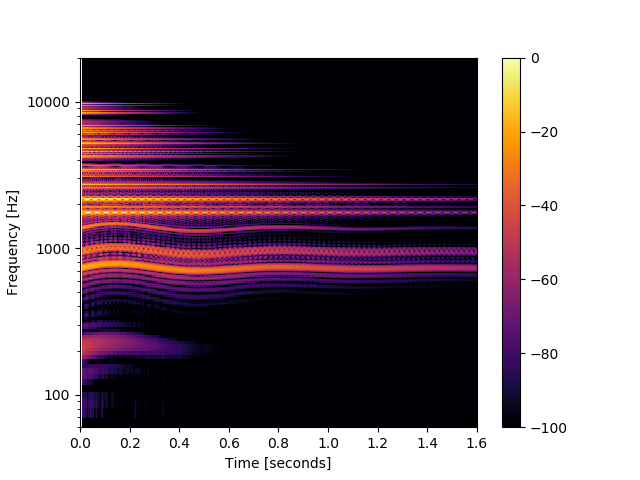
\includegraphics[width=\linewidth,trim={0 0 1cm 1cm},clip]{../Figures/Specgrams/Vibrato.png}
    \caption{\it{A spectrogram of a synthesized waterbottle with exaggerated swinging vibrato on the lowest five modes.}}
    \label{fig:swinging-vibrato}
\end{figure}

%
\subsection{Impact Analysis} \label{sec:impact}
%
In real-world situations, a water bottle is typically struck using a body part
(knee, elbow, knuckles, etc), or using a striker that can be easily found in
nature, for instance a stick. With the goal of being able to synthesize these
types of impacts, we used an accelerometer to measure the impacts of
several body parts, as well as several types of drumsticks on a water bottle.
\Cref{fig:impact} shows the time and frequency domain
measurements of the various impact types. We can use any of these measurements as the input $x(t)$ in \eqref{eq:phasor} to synthesize the sound of a water bottle struck by the desired striker.

\begin{figure}[t]
\centering
    \begin{subfigure}[b]{\columnwidth}
         \centering
         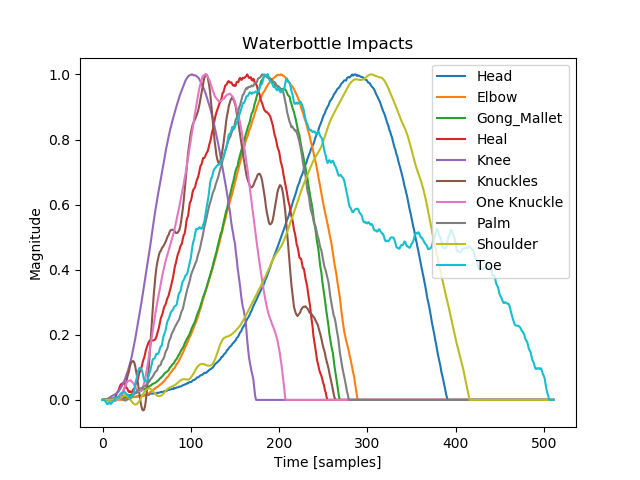
\includegraphics[width=\linewidth,trim={0 0 1cm 1cm},clip]{../Figures/Impacts_time}
         \caption{Time Domain}
    \end{subfigure}
    \begin{subfigure}[b]{\columnwidth}
         \centering
         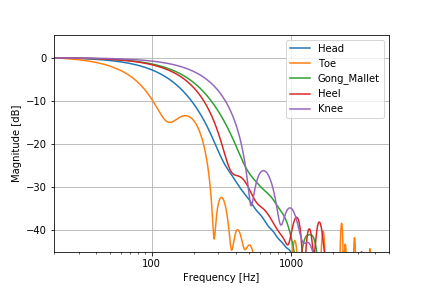
\includegraphics[width=\linewidth,trim={0 0 1cm 1cm},clip]{../Figures/Impacts_freq}
         \caption{Frequency Domain}
    \end{subfigure}
    \caption{\it{Time and frequency domain measurements of various impact drives.}}
    \label{fig:impact}
\end{figure}


\section{Results} \label{sec:results}
%
While one may expect the acoustic profile of the humble water bottle to be dramatically simple, the measurements and analysis presented here demonstrate how significantly the sound changes when the water bottle is filled by different amounts of water and covered by different amounts of stickers. 

%
\subsection{Water Bottle Synthesizers} \label{sec:synth}

\subsubsection{HydroFlask Synthesizer}
To demonstrate the musical power of water bottle synthesis, we have
implemented a modal model of the 32 Oz. Wide Mouth HydroFlask
as an 8-voice synthesizer plugin (VST/AU), using the JUCE/C++
framework (see \Cref{fig:plugin}).\footnote{\url{https://github.com/weAreROLI/JUCE}}
The synthesizer includes controls for the amount of water in the bottle,
the number and placement of stickers on the bottle, and the option to
strike the water bottle with a variety of objects. 

\subsubsection{Bespoke Water bottle Synthesizers}
Water bottles are often cherished possessions---potentially partially due to the unique sound of a well-loved water bottle covered in memorable stickers and dents. In an effort to expand the world of water bottle synthesis to a wider
audience, we have developed a system for creating a ``bespoke''
water bottle synthesizer for any water bottle. The first part of the
system is comprised of a web app\footnote{\url{http://ccrmawaterbottles.pythonanywhere.com/}}
containing the modal analysis algorithm defined in \S\ref{sec:modal-analysis}. 
Here users can upload their own water bottle recordings, and can download a
\texttt{.waterbottle} file containing the modal characteristics of the
recording that was uploaded. All water bottle characteristics are saved in 
a database. The second part of the system is comprised of
a second audio plugin that can recreate a modal water bottle synthesizer
(including variable strikers and water amounts) from any \texttt{.waterbottle}
file. Users can then download the modal characteristics of any water
bottle in the database and use it in their synthesizer.
%
\begin{figure}
    \centering
    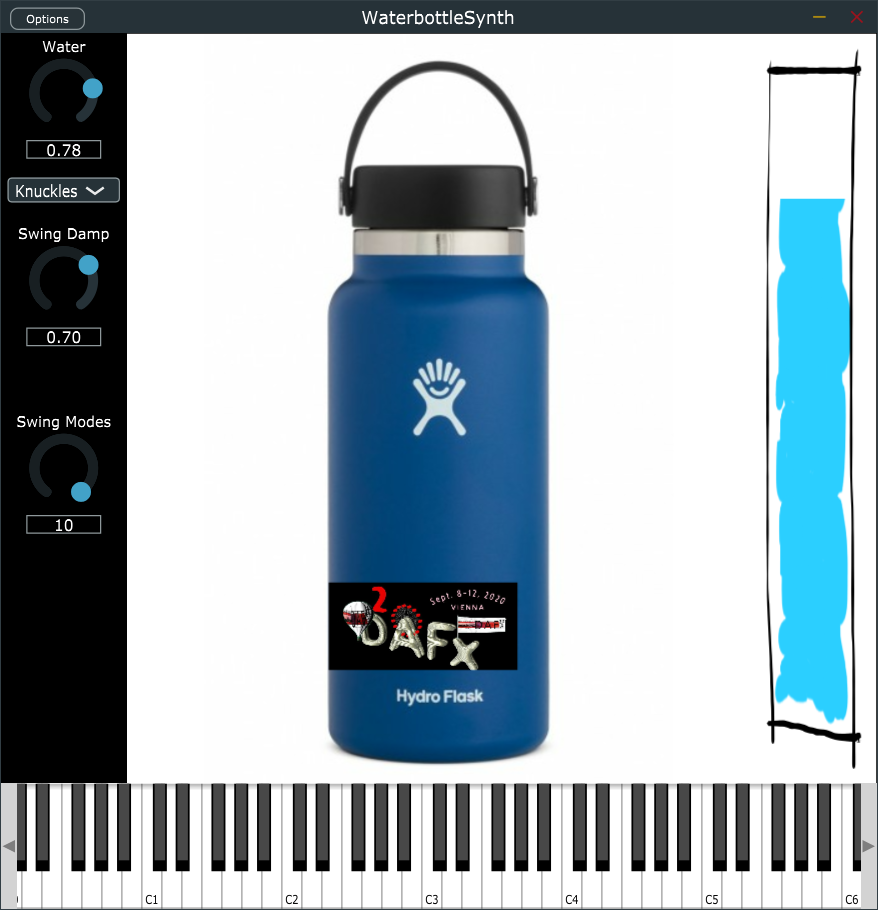
\includegraphics[width=3in]{../Figures/WaterbottleSynthPlugin.png}
    \caption{\it{Real-time modal synthesizer model of the HydroFlask
    32 oz. Wide Mouth.}}
    \label{fig:plugin}
\end{figure}

Video demos of each plugin can be found on
YouTube,\footnote{\url{https://youtu.be/MwhBluJqePE}}
and the source code for both plugins, as well as all the modal
analysis described in the paper is publicly available on
GitHub.\footnote{\url{https://github.com/jatinchowdhury18/modal-waterbottles}}
Audio samples of various synthesized water bottles discussed in this
writing can be found online.\footnote{\url{https://ccrma.stanford.edu/~jatin/Waterbottles}}

%
\section{Conclusion} \label{sec:conclusion}
%
We have discussed the synthesis of water bottle acoustics
using modal signal processing techniques. We have described the processes
of making acoustic measurements of the water bottles, as well as performing
modal analysis, with specific considerations for the amount of water
contained in the bottle, as well as the stickers placed on the exterior
of the bottle. Finally, we have implemented our modal model of a 32 oz.
Wide Mouth HydroFlask bottle as a real-time synthesizer plugin.
\newline\newline
Future research in this area concerns the extension of water bottle
modelling to include a wider range of bottles, with various sizes and
shapes, and made of various materials. For high-end water bottle
manufacturers, acoustic analysis could be used to improve the sound
of their water bottles. Extended research goals include the creation
of a physical, musically-tuned water bottle xylophone, as well as potentially
determining the optimally acoustic water bottle currently in production.

\section{Acknowledgements}
%
The authors would like to thank Eric Lawrence at Polytec for inviting us to use the scanning vibrometer and Kim Kawczinski for helping us to contact
the HydroFlask corporation.

%\newpage
\nocite{*}
\bibliographystyle{IEEEbib}
\bibliography{references}

\end{document}
